\begin{enumerate}[label=\thesubsection.\arabic*, ref=\thesubsection.\theenumi]
	
	\item Evaluate:
	\begin{align*}
		\lim_{x \to 0} \frac{e^x - 1}{\sqrt{1 - \cos x}}
	\end{align*}
	\solution
	From \eqref{eq:exp_taylor} and \eqref{eq:half_angle_cos}:
	\begin{align}
		\lim_{x \to 0} \frac{1 + x + O(x^2) - 1}{\sqrt{2\sin^2\brak{\frac{x}{2}}}} &= \lim_{x \to 0} \frac{x}{\sqrt{2}\abs{\sin\brak{\frac{x}{2}}}}
	\end{align}
	Evaluating the one-sided limits:
	\begin{align}
		\lim_{x \to 0^+} \frac{x}{\sqrt{2}\sin\brak{\frac{x}{2}}} &= \sqrt{2}, \quad \lim_{x \to 0^-} \frac{x}{-\sqrt{2}\sin\brak{\frac{x}{2}}} = -\sqrt{2}
	\end{align}
	Since the left-hand and right-hand limits are not equal, the limit does not exist.
	\begin{figure}[H]
		\centering
		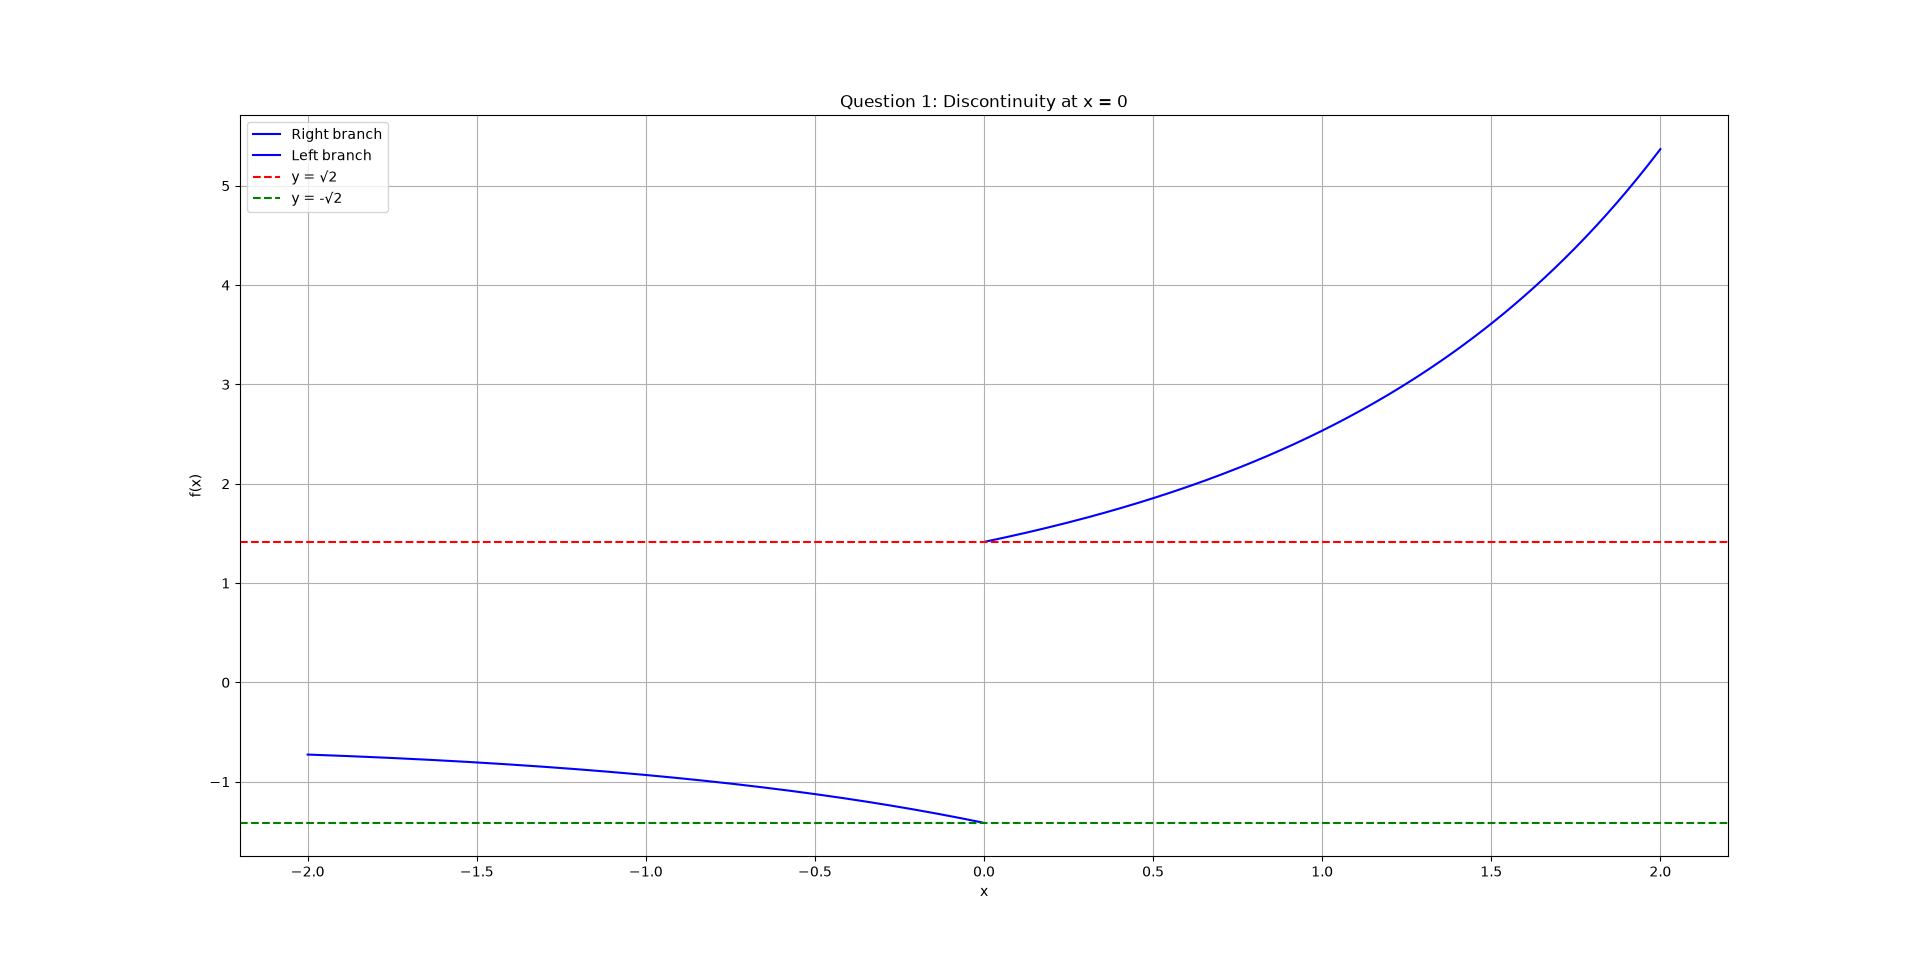
\includegraphics[width=0.6\textwidth]{figs/q1_fig}
		\caption{Discontinuity and one-sided limits at $x = 0$.}
		\label{fig:q1_fig}
		\vspace{0.5em}
		\noindent\fbox{\parbox{\dimexpr\linewidth-2\fboxsep-2\fboxrule}{\hspace{2em}\textbackslash codes\textbackslash q1.py}}
	\end{figure}
	
	\item Solve the differential equation $x\frac{dy}{dx} + y = x^3$, given $y=1$ when $x=2$.
	
	\solution
	Applying the Laplace Transform $\mathcal{L}\{y(x)\} = Y(s)$ using the derivative and $x$-multiplication properties from \eqref{eq:laplace_diff_rules}:
	\begin{align}
		\mathcal{L}\cbrak{x\frac{dy}{dx}} + \mathcal{L}\cbrak{y} &= \mathcal{L}\cbrak{x^3} \\
		-\frac{d}{ds}\sbrak{sY(s) - y(0)} + Y(s) &= \frac{3!}{s^4}
	\end{align}
	Expanding the derivative in the $s$-domain:
	\begin{align}
		-\sbrak{Y(s) + s\frac{dY}{ds}} + Y(s) = \frac{6}{s^4} \implies -s\frac{dY}{ds} = \frac{6}{s^4} \implies \frac{dY}{ds} = -\frac{6}{s^5}
	\end{align}
	Integrating with respect to $s$:
	\begin{align}
		Y(s) = \int -\frac{6}{s^5} \, ds = \frac{3}{2s^4} + C_1
	\end{align}
	Since $\lim_{s \to \infty} Y(s) = 0$, $C_1 = 0$. Taking the inverse Laplace transform and including the homogeneous solution $\frac{C}{x}$ for the singularity at $x = 0$:
	\begin{align}
		y(x) = \mathcal{L}^{-1}\cbrak{\frac{1}{4}\cdot\frac{3!}{s^4}} + \frac{C}{x} = \frac{x^3}{4} + \frac{C}{x} \label{eq:de_sol_gen}
	\end{align}
	Substituting the initial condition $\vec{x}_0 = \myvec{2 \\ 1}$ into \eqref{eq:de_sol_gen}:
	\begin{align}
		1 = \frac{2^3}{4} + \frac{C}{2} \implies 1 = 2 + \frac{C}{2} \implies C = -2
	\end{align}
	Substituting $C = -2$ yields the particular solution:
	\begin{align}
		y = \frac{x^3}{4} - \frac{2}{x}
	\end{align}
	
	\item Given $\vec{A} = \myvec{3 & -2 \\ 4 & -2}$, find $k$ such that $\vec{A}^2 = k\vec{A} - 2\vec{I}_2$.
	
	\solution
	Computing $\vec{A}^2$:
	\begin{align}
		\vec{A}^2 = \myvec{3 & -2 \\ 4 & -2}\myvec{3 & -2 \\ 4 & -2} = \myvec{1 & -2 \\ 4 & -4}
	\end{align}
	By the Cayley-Hamilton theorem in \eqref{eq:cayley_hamilton_formula}:
	\begin{align}
		\vec{A}^2 - \text{Tr}(\vec{A})\vec{A} + \mydet{\vec{A}}\vec{I}_2 = \vec{0}
	\end{align}
	Evaluating the trace and determinant of $\vec{A}$:
	\begin{align}
		\text{Tr}(\vec{A}) = 3 + (-2) = 1, \quad \mydet{\vec{A}} = (3)(-2) - (-2)(4) = 2
	\end{align}
	Substituting these values:
	\begin{align}
		\vec{A}^2 - \vec{A} + 2\vec{I}_2 = \vec{0} \implies \vec{A}^2 = \vec{A} - 2\vec{I}_2
	\end{align}
	Comparing with $\vec{A}^2 = k\vec{A} - 2\vec{I}_2$ yields $k = 1$.
	
	\item Using the properties of determinants, show that:
	\begin{align*}
		\mydet{a+x & y & a+z \\ z & a+y & z \\ z & y & a+z} = a^2(a+x+y+z)
	\end{align*}
	\solution
	By standard determinant operations referenced in \eqref{eq:det_prop_identity}:
	\begin{align}
		\mydet{a+x & y & a+z \\ z & a+y & z \\ z & y & a+z} 
		&\xrightarrow{R_1 \to R_1 - R_3} \mydet{a+x-z & 0 & 0 \\ z & a+y & z \\ z & y & a+z} \\
		&= (a+x-z)\mydet{a+y & z \\ y & a+z} \\
		&\xrightarrow{C_1 \to C_1 - C_2} (a+x-z)\mydet{a+y-z & z \\ 0 & a+z}
	\end{align}
	Alternatively:
	\begin{align}
		\mydet{a+x & y & a+z \\ z & a+y & z \\ z & y & a+z} 
		&\xrightarrow{R_1 \to R_1 + R_2 + R_3} \mydet{a+x+2z & a+2y & a+2z+y \\ z & a+y & z \\ z & y & a+z} \\
		&\xrightarrow{\substack{R_1 \to R_1 - R_3 \\ R_2 \to R_2 - R_3}} \mydet{a+x & 0 & 0 \\ 0 & a & 0 \\ z & y & a+z} \\
		&= a^2(a+x+y+z)
	\end{align}
	
	\item Find the intervals on which the function $f(x) = \frac{x}{1+x^2}$ is
	
	(a) Increasing
	
	(b) Decreasing.
	
	\solution
	Differentiating $f(x)$ with respect to $x$:
	\begin{align}
		f'(x) = \frac{(1+x^2)(1) - x(2x)}{(1+x^2)^2} = \frac{1 - x^2}{(1+x^2)^2}
	\end{align}
	Applying the monotonicity criteria from \eqref{eq:monotonicity_cond}:
	\begin{enumerate}[label=(\alph*)]
		\item For $f(x)$ to be increasing, $f'(x) \ge 0 \implies 1 - x^2 \ge 0 \implies x \in [-1, 1]$.
		\item For $f(x)$ to be decreasing, $f'(x) \le 0 \implies 1 - x^2 \le 0 \implies x \in (-\infty, -1] \cup [1, \infty)$.
	\end{enumerate}
	\begin{figure}[H]
		\centering
		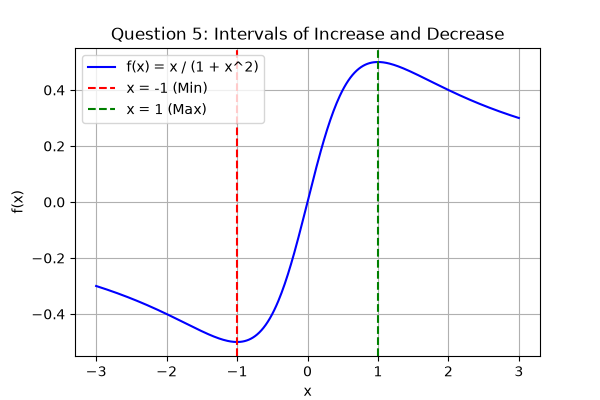
\includegraphics[width=0.7\textwidth]{figs/q5_fig}
		\caption{Intervals of increase and decrease for $f(x) = \frac{x}{1+x^2}$.}
		\label{fig:q5_fig}
		\vspace{0.5em}
		\noindent\fbox{\parbox{\dimexpr\linewidth-2\fboxsep-2\fboxrule}{\hspace{2em}\textbackslash codes\textbackslash q5.py}}
	\end{figure}
	
	\item \hfill
	\begin{enumerate}[label=(\alph*)]
		\item Approximate $I = \int_{0}^{\pi/2} \frac{\sin^2 x}{\sin x + \cos x} dx$ using the Trapezoidal Rule with $N=4$ subintervals.
		\item Approximate $I = \int_{0}^{\pi} \frac{x \sin x}{1 + \cos^2 x} dx$ using the Trapezoidal Rule with $N=4$ subintervals.
	\end{enumerate}
	\solution
	\begin{figure}[H]
		\centering
		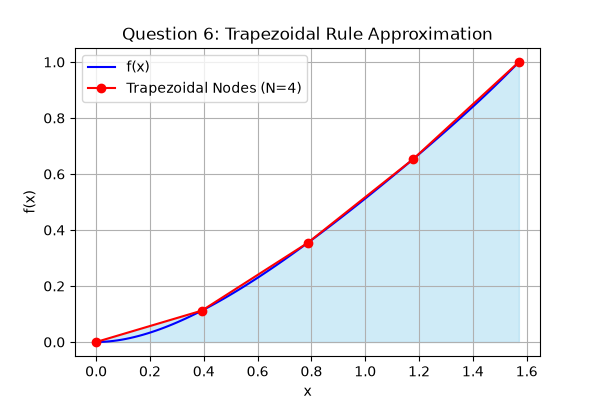
\includegraphics[width=0.7\textwidth]{figs/q6_fig}
		\caption{Trapezoidal Rule integration nodes.}
		\label{fig:q6_fig}
		\vspace{0.5em}
		\noindent\fbox{\parbox{\dimexpr\linewidth-2\fboxsep-2\fboxrule}{\hspace{2em}\textbackslash codes\textbackslash q6.py}}
	\end{figure}
	\begin{enumerate}[label=(\alph*)]
		\item Applying the Trapezoidal Rule formula from \eqref{eq:trapezoidal_rule} with $h = \frac{\pi/2 - 0}{4} = \frac{\pi}{8}$:
		Evaluating $f(x) = \frac{\sin^2 x}{\sin x + \cos x}$ at nodes $x_k = \frac{k\pi}{8}$ for $k=0,1,2,3,4$:
		\begin{align}
			y_0 &= f(0) = 0, \quad y_1 = f\brak{\frac{\pi}{8}} \approx 0.1118 \\
			y_2 &= f\brak{\frac{\pi}{4}} \approx 0.3536, \quad y_3 = f\brak{\frac{3\pi}{8}} \approx 0.6010, \quad y_4 = f\brak{\frac{\pi}{2}} = 1.0000
		\end{align}
		Applying \eqref{eq:trapezoidal_rule}:
		\begin{align}
			I &\approx \frac{\pi}{16} \sbrak{y_0 + 2(y_1 + y_2 + y_3) + y_4} \approx 0.6151
		\end{align}
		\item Applying \eqref{eq:trapezoidal_rule} with $h = \frac{\pi}{4}$:
		Evaluating $g(x) = \frac{x\sin x}{1+\cos^2 x}$ at nodes $x_k = \frac{k\pi}{4}$ for $k=0,1,2,3,4$:
		\begin{align}
			y_0 = 0, \quad y_1 \approx 0.3702, \quad y_2 \approx 1.5708, \quad y_3 \approx 1.1107, \quad y_4 = 0
		\end{align}
		Applying \eqref{eq:trapezoidal_rule}:
		\begin{align}
			I &\approx \frac{\pi}{8} \sbrak{y_0 + 2(y_1 + y_2 + y_3) + y_4} \approx 2.3968
		\end{align}
	\end{enumerate}
	
	\item Find Karl Pearson's coefficient of correlation between $x$ and $y$ for the given data vectors:
	\begin{align*}
		\vec{x} = \myvec{10 \\ 7 \\ 12 \\ 15 \\ 9 \\ 15 \\ 8}, \quad \vec{y} = \myvec{6 \\ 4 \\ 7 \\ 10 \\ 11 \\ 8 \\ 10}
	\end{align*}
	\solution
	Applying Karl Pearson's correlation coefficient in vector notation from \eqref{eq:karl_pearson_vec}:
	Computing the mean vectors using $\vec{1} = \myvec{1 & 1 & 1 & 1 & 1 & 1 & 1}^{\top}$:
	\begin{align}
		\bar{x} = \frac{\vec{1}^{\top}\vec{x}}{7} = \frac{76}{7} \approx 10.86, \quad \bar{y} = \frac{\vec{1}^{\top}\vec{y}}{7} = \frac{56}{7} = 8
	\end{align}
	Forming centered vectors $\vec{u} = \vec{x} - \bar{x}\vec{1}$ and $\vec{v} = \vec{y} - \bar{y}\vec{1}$:
	\begin{align}
		\vec{u}^{\top}\vec{v} = 22, \quad \norm{\vec{u}}^2 = 64.86, \quad \norm{\vec{v}}^2 = 42
	\end{align}
	Evaluating Karl Pearson's coefficient:
	\begin{align}
		r = \frac{\vec{u}^{\top}\vec{v}}{\norm{\vec{u}}\norm{\vec{v}}} = \frac{22}{\sqrt{64.86 \times 42}} \approx 0.421
	\end{align}
	
	\item A bag contains 8 red, 3 white, and 9 blue balls. If three balls are drawn at random, determine the probability that:
	
	(a) All three balls are blue
	
	(b) All balls are of different colors.
	
	\solution
	Expressing probability using Probability Mass Functions (PMF) $p_X(k) = \pr{X = k}$ as per \eqref{eq:pmf_prob_def}:
	Total sample space size $N = \comb{20}{3} = 1140$.
	\begin{enumerate}[label=(\alph*)]
		\item For $X = 3$ blue balls:
		\begin{align}
			p_X(3) = \frac{\comb{9}{3}\comb{11}{0}}{\comb{20}{3}} = \frac{84}{1140} = \frac{7}{95}
		\end{align}
		\item For $Y = (1\text{R}, 1\text{W}, 1\text{B})$:
		\begin{align}
			p_Y(1\text{R}, 1\text{W}, 1\text{B}) = \frac{\comb{8}{1} \times \comb{3}{1} \times \comb{9}{1}}{\comb{20}{3}} = \frac{216}{1140} = \frac{18}{95}
		\end{align}
	\end{enumerate}
	
	\item In a single throw of two dice, find the probability that neither a doublet nor a total of 10 will appear.
	
	\solution
	Define sample space size $N = 36$. Let $X = \mathbb{I}(\text{doublet or sum}=10)$.
	Using PMF formulation from \eqref{eq:pmf_prob_def}:
	\begin{align}
		p_X(1) = \pr{A \cup B} = \frac{6}{36} + \frac{3}{36} - \frac{1}{36} = \frac{8}{36} = \frac{2}{9}
	\end{align}
	The PMF for neither event occurring ($X = 0$) is:
	\begin{align}
		p_X(0) = 1 - p_X(1) = 1 - \frac{2}{9} = \frac{7}{9}
	\end{align}
	
	\item Using Gauss Elimination method, solve the system of linear equations:
	\begin{align*}
		2x - y + z &= -3 \\
		3x - z &= -8 \\
		2x + 6y &= 2
	\end{align*}
	\solution
	Constructing the augmented matrix $[\vec{A} | \vec{b}]$ as defined in \eqref{eq:gauss_elimination_def}:
	\begin{align}
		\left[\begin{array}{ccc|c}
			2 & -1 & 1 & -3 \\
			3 & 0 & -1 & -8 \\
			2 & 6 & 0 & 2
		\end{array}\right]
	\end{align}
	Applying row operations $R_2 \to R_2 - \frac{3}{2}R_1$ and $R_3 \to R_3 - R_1$, followed by $R_3 \to R_3 - \frac{14}{3}R_2$:
	\begin{align}
		\left[\begin{array}{ccc|c}
			2 & -1 & 1 & -3 \\
			0 & 1.5 & -2.5 & -3.5 \\
			0 & 0 & \frac{32}{3} & \frac{64}{3}
		\end{array}\right]
	\end{align}
	Back-substitution yields $z = 2, y = 1, x = -2 \implies \vec{x} = \myvec{-2 \\ 1 \\ 2}$.
	
	\item Prove that the area enclosed by $y^2 = 4ax$ and $x^2 = 4ay$ is $\frac{16}{3}a^2$ square units.
	
	\solution
	\begin{figure}[H]
		\centering
		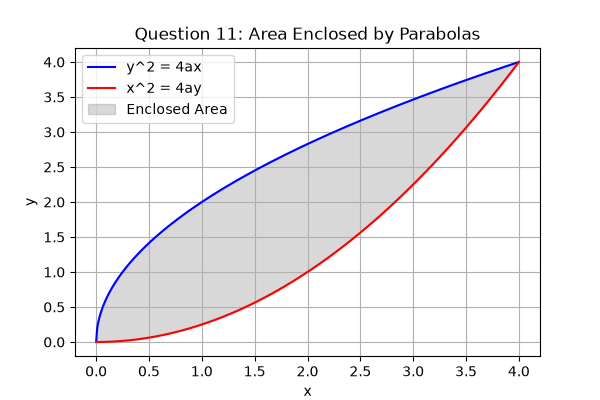
\includegraphics[width=0.7\textwidth]{figs/q11_fig}
		\caption{Area enclosed between the parabolas $y^2 = 4ax$ and $x^2 = 4ay$.}
		\label{fig:q11_fig}
		\vspace{0.5em}
		\noindent\fbox{\parbox{\dimexpr\linewidth-2\fboxsep-2\fboxrule}{\hspace{2em}\textbackslash codes\textbackslash q11.py}}
	\end{figure}
	Solving the intersection points of the two parabolas:
	\begin{align}
		\brak{\frac{x^2}{4a}}^2 = 4ax \implies x^4 = 64a^3x \implies x(x^3 - 64a^3) = 0 \implies x = 0, \, x = 4a
	\end{align}
	The area enclosed between $x = 0$ and $x = 4a$ is:
	\begin{align}
		\text{Area} &= \int_{0}^{4a} \brak{\sqrt{4ax} - \frac{x^2}{4a}} dx = \sbrak{2\sqrt{a}\cdot\frac{2}{3}x^{3/2} - \frac{x^3}{12a}}_{0}^{4a} \nonumber \\
		&= \frac{4}{3}\sqrt{a}(8a^{3/2}) - \frac{64a^3}{12a} = \frac{32}{3}a^2 - \frac{16}{3}a^2 = \frac{16}{3}a^2 \quad \text{sq. units} \label{eq:area_parabolas}
	\end{align}
	
	\item \hfill
	\begin{enumerate}[label=(\alph*)]
		\item Using vectors prove that $\cos A = \frac{b^2 + c^2 - a^2}{2bc}$.
		\item Three bags contain balls as shown in the following table:
		\begin{center}
			\begin{tabular}{|c|c|c|c|}
				\hline
				Bag & \multicolumn{3}{c|}{Number of} \\ \hline
				& White balls & Black balls & Red balls \\ \hline
				I & 1 & 2 & 3 \\
				II & 2 & 1 & 1 \\
				III & 4 & 3 & 2 \\ \hline
			\end{tabular}
		\end{center}
		A bag is chosen at random and two balls are drawn. They happen to be white and red. What is the probability that they came from the third bag?
	\end{enumerate}
	\solution
	\begin{figure}[H]
		\centering
		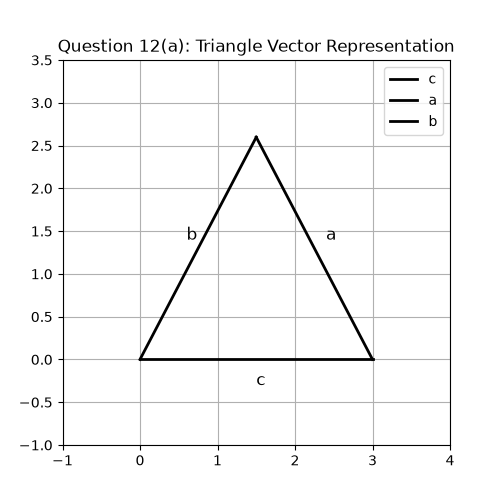
\includegraphics[width=0.6\textwidth]{figs/q12_fig}
		\caption{Triangle side vectors for the law of cosines proof.}
		\label{fig:q12_fig}
		\vspace{0.5em}
		\noindent\fbox{\parbox{\dimexpr\linewidth-2\fboxsep-2\fboxrule}{\hspace{2em}\textbackslash codes\textbackslash q12.py}}
	\end{figure}
	\begin{enumerate}[label=(\alph*)]
		\item Let the side vectors of triangle $ABC$ be related by $\vec{a} + \vec{b} + \vec{c} = \vec{0} \implies \vec{a} = -\brak{\vec{b} + \vec{c}}$. Taking the dot product of $\vec{a}$ with itself:
		\begin{align}
			\norm{\vec{a}}^2 &= \brak{\vec{b} + \vec{c}}^{\top}\brak{\vec{b} + \vec{c}} \\
			a^2 &= \norm{\vec{b}}^2 + \norm{\vec{c}}^2 + 2\vec{b}^{\top}\vec{c} \\
			a^2 &= b^2 + c^2 - 2bc\cos A
		\end{align}
		Rearranging yields:
		\begin{align}
			\cos A = \frac{b^2 + c^2 - a^2}{2bc}
		\end{align}
		\item Prior PMF $p_B(1) = p_B(2) = p_B(3) = \frac{1}{3}$.
		Conditional PMFs for drawing 1 white and 1 red ball $E$:
		\begin{align}
			p_{E|B}(e|1) = \frac{1}{5}, \quad p_{E|B}(e|2) = \frac{1}{3}, \quad p_{E|B}(e|3) = \frac{2}{9}
		\end{align}
		Applying Bayes' Theorem PMF formulation:
		\begin{align}
			p_{B|E}(3|e) = \frac{\frac{1}{3} \times \frac{2}{9}}{\frac{1}{3}\brak{\frac{1}{5} + \frac{1}{3} + \frac{2}{9}}} = \frac{\frac{2}{9}}{\frac{34}{45}} = \frac{5}{17}
		\end{align}
	\end{enumerate}
	
	\item The first four moments of a distribution about $x=2$ are $1, 2.5, 5.5$, and $16$ respectively. Calculate the four moments about the mean.
	
	\solution
	Given raw moments $\mu_1' = 1, \mu_2' = 2.5, \mu_3' = 5.5, \mu_4' = 16$ about $A = 2$.
	The central moments $\mu_r$ about the mean are:
	\begin{align}
		\mu_1 &= 0 \\
		\mu_2 &= \mu_2' - (\mu_1')^2 = 2.5 - (1)^2 = 1.5 \\
		\mu_3 &= \mu_3' - 3\mu_2'\mu_1' + 2(\mu_1')^3 = 5.5 - 7.5 + 2 = 0 \\
		\mu_4 &= \mu_4' - 4\mu_3'\mu_1' + 6\mu_2'(\mu_1')^2 - 3(\mu_1')^4 = 16 - 22 + 15 - 3 = 6
	\end{align}
	Central moments: $\mu_1 = 0, \mu_2 = 1.5, \mu_3 = 0, \mu_4 = 6$.
	
	\item \hfill
	\begin{enumerate}[label=(\alph*)]
		\item A particle is projected so as to graze the tops of two walls, each of height $10\text{ m}$ at distances $15\text{ m}$ and $45\text{ m}$ respectively from the point of projection. Prove that the angle of projection is $\tan^{-1}\brak{\frac{8}{9}}$.
		\item A starts a business with a capital of Rs. $4,00,000$. After 3 months B joins him with a capital of Rs. $6,00,000$ and at the end of another 3 months C joins with Rs. $10,00,000$. If at the end of the year, the total profit be Rs. $5,40,000$, and they share it in the ratio of their effective capitals, calculate the shares of A, B and C in the total profit.
	\end{enumerate}
	\solution
	\begin{enumerate}[label=(\alph*)]
		\item Using the trajectory formula from \eqref{eq:projectile_trajectory}:
		\begin{align}
			y = x \tan\theta \brak{1 - \frac{x}{R}}
		\end{align}
		Since the particle grazes two walls of height $h = 10\text{ m}$ at $x_1 = 15\text{ m}$ and $x_2 = 45\text{ m}$:
		\begin{align}
			10 &= 15 \tan\theta \brak{1 - \frac{15}{R}} \label{eq:wall1} \\
			10 &= 45 \tan\theta \brak{1 - \frac{45}{R}} \label{eq:wall2}
		\end{align}
		Equating \eqref{eq:wall1} and \eqref{eq:wall2}:
		\begin{align}
			15 \brak{1 - \frac{15}{R}} = 45 \brak{1 - \frac{45}{R}} \implies 1 - \frac{15}{R} = 3 - \frac{135}{R} \implies \frac{120}{R} = 2 \implies R = 60\text{ m}
		\end{align}
		Substituting $R = 60\text{ m}$ into \eqref{eq:wall1}:
		\begin{align}
			10 = 15 \tan\theta \brak{1 - \frac{15}{60}} = 15 \tan\theta \brak{\frac{3}{4}} = \frac{45}{4}\tan\theta \implies \tan\theta = \frac{40}{45} = \frac{8}{9}
		\end{align}
		Thus, the angle of projection is $\theta = \tan^{-1}\brak{\frac{8}{9}}$.
		\begin{figure}[H]
			\centering
			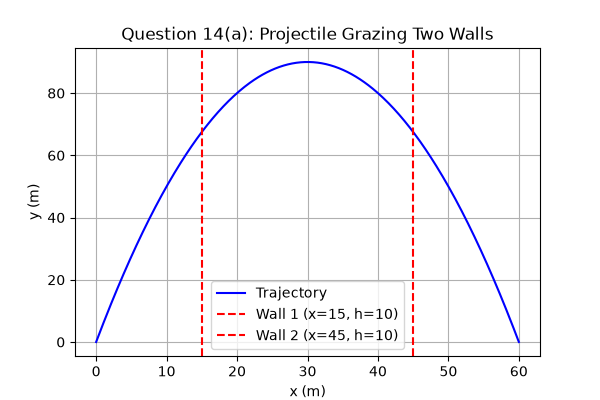
\includegraphics[width=0.7\textwidth]{figs/q14_fig}
			\caption{Projectile trajectory grazing two walls.}
			\label{fig:q14_fig}
			\vspace{0.5em}
			\noindent\fbox{\parbox{\dimexpr\linewidth-2\fboxsep-2\fboxrule}{\hspace{2em}\textbackslash codes\textbackslash q14.py}}
		\end{figure}
		\item Effective capital-months vector $\vec{c} = \myvec{48,00,000 \\ 54,00,000 \\ 60,00,000} \implies \vec{r} = \myvec{8 \\ 9 \\ 10}$.
		Sum of ratio terms $\vec{1}^{\top}\vec{r} = 27$.
		Profit vector $\vec{p} = \frac{5,40,000}{27}\myvec{8 \\ 9 \\ 10} = \myvec{1,60,000 \\ 1,80,000 \\ 2,00,000}$.
		Shares: A $=$ Rs. $1,60,000$, B $=$ Rs. $1,80,000$, C $=$ Rs. $2,00,000$.
	\end{enumerate}
	
	\item \hfill
	\begin{enumerate}[label=(\alph*)]
		\item A stone is projected vertically upward with a velocity sufficient to carry it to a height of $50\text{ m}$. Find its velocity of projection and the time taken to come back to the ground. [Use $g = 9.8\text{ m/s}^2$]
		\item The cost function of a firm is given by $C(x) = 300x - 10x^2 + \frac{x^3}{3}$. Calculate the output at which the marginal cost is minimum. Also calculate the minimum marginal cost.
	\end{enumerate}
	\solution
	\begin{enumerate}[label=(\alph*)]
		\item Applying the vertical motion formulas under gravity from \eqref{eq:vertical_motion_gravity}:
		Given maximum height $H = 50\text{ m}$ and acceleration due to gravity $g = 9.8\text{ m/s}^2$.
		At the highest point, final velocity $v = 0$:
		\begin{align}
			v^2 = u^2 - 2gH \implies 0 = u^2 - 2(9.8)(50) \implies u^2 = 980 \implies u = \sqrt{980} = 14\sqrt{5} \approx 31.30\text{ m/s}
		\end{align}
		The total time taken to return to the ground (time of flight $T$):
		\begin{align}
			T = \frac{2u}{g} = \frac{2 \times 31.3049}{9.8} \approx 6.39\text{ seconds}
		\end{align}
		\begin{figure}[H]
			\centering
			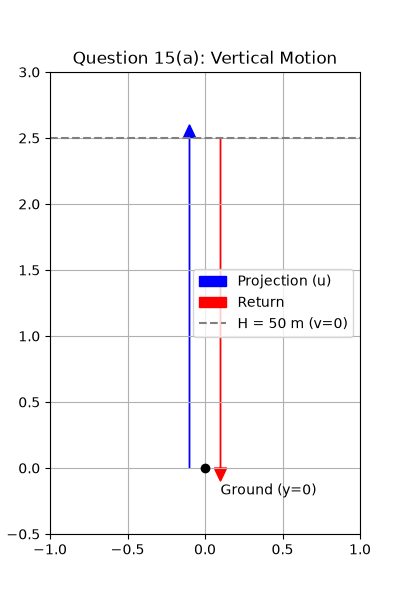
\includegraphics[width=0.5\textwidth]{figs/q15_fig}
			\caption{Vertical motion under gravity.}
			\label{fig:q15_fig}
			\vspace{0.5em}
			\noindent\fbox{\parbox{\dimexpr\linewidth-2\fboxsep-2\fboxrule}{\hspace{2em}\textbackslash codes\textbackslash q15.py}}
		\end{figure}
		\item Marginal Cost $MC = \frac{dC}{dx} = 300 - 20x + x^2$.
		Minimizing $MC$: $\frac{d(MC)}{dx} = -20 + 2x = 0 \implies x = 10$.
		Since $\frac{d^2(MC)}{dx^2} = 2 > 0$, $MC$ is minimum at $x = 10$.
		$MC_{\text{min}} = 300 - 20(10) + (10)^2 = 200$.
	\end{enumerate}
	
	\item \hfill
	\begin{enumerate}[label=(\alph*)]
		\item Solve the differential equation $\frac{d^2y}{dx^2} = \log x$, given that $x=1, y=1 \text{ and } \frac{dy}{dx} = 1$.
		\item Calculate Bowley's coefficient of skewness for the given frequency distribution:
		\begin{center}
			\begin{tabular}{|c|c|c|c|c|c|c|c|c|c|}
				\hline
				x & 5 & 10 & 15 & 20 & 25 & 30 & 35 & 40 & 45 \\ \hline
				y & 9 & 8 & 12 & 15 & 11 & 7 & 6 & 5 & 2 \\ \hline
			\end{tabular}
		\end{center}
	\end{enumerate}
	\solution
	\begin{enumerate}[label=(\alph*)]
		\item Applying the Laplace Transform $\mathcal{L}\{y(x)\} = Y(s)$ using the derivative property from \eqref{eq:laplace_diff_rules}:
		\begin{align}
			\mathcal{L}\cbrak{\frac{d^2y}{dx^2}} &= \mathcal{L}\cbrak{\log x} \\
			s^2 Y(s) - s y(0) - y'(0) &= -\frac{\gamma + \log s}{s}
		\end{align}
		where $\gamma$ is the Euler-Mascheroni constant. Dividing by $s^2$:
		\begin{align}
			Y(s) = \frac{y(0)}{s} + \frac{y'(0)}{s^2} - \frac{\gamma + \log s}{s^3}
		\end{align}
		Using the inverse Laplace transform $\mathcal{L}^{-1}\cbrak{-\frac{\gamma + \log s}{s^3}} = \frac{x^2}{2}\log x - \frac{3x^2}{4}$:
		\begin{align}
			y(x) = y(0) + y'(0)x + \frac{x^2}{2}\log x - \frac{3x^2}{4}
		\end{align}
		Letting $C_1 = y'(0)$ and $C_2 = y(0)$ for the boundary conditions at $x = 1$:
		\begin{align}
			y(x) &= \frac{x^2}{2}\log x - \frac{3x^2}{4} + C_1 x + C_2 \label{eq:q16a_gen} \\
			\frac{dy}{dx} &= x\log x - x + C_1 \label{eq:q16a_diff}
		\end{align}
		Substituting $x = 1, \frac{dy}{dx} = 1$ into \eqref{eq:q16a_diff}:
		\begin{align}
			1 = 1\log(1) - 1 + C_1 \implies C_1 = 2
		\end{align}
		Substituting $x = 1, y = 1$ and $C_1 = 2$ into \eqref{eq:q16a_gen}:
		\begin{align}
			1 = 0 - \frac{3}{4} + 2(1) + C_2 \implies C_2 = -\frac{1}{4}
		\end{align}
		Thus, the particular solution is:
		\begin{align}
			y = \frac{x^2}{2}\log x - \frac{3x^2}{4} + 2x - \frac{1}{4}
		\end{align}
		\item Constructing cumulative frequency ($N = 75$):
		Quartile positions give $Q_1 = 15, Q_2 = 20, Q_3 = 30$.
		Bowley's coefficient $S_b = \frac{Q_3 + Q_1 - 2Q_2}{Q_3 - Q_1} = \frac{30 + 15 - 40}{30 - 15} = \frac{5}{15} = \frac{1}{3} \approx 0.333$.
	\end{enumerate}
	
	\item \hfill
	\begin{enumerate}[label=(\alph*)]
		\item The Cartesian equations of a line are $6x - 2 = 3y + 1 = 2z - 2$. Find:
		\begin{enumerate}[label=(\roman*)]
			\item The direction ratios of the line.
			\item Cartesian and vector equations of the line parallel to this line and passing through the point $(2, -1, -1)$.
		\end{enumerate}
		\item Find the present value of an ordinary annuity of Rs. $500$ per annum for $12$ years at $15\%$ per annum. [Given $(1.15)^{-12} = \frac{1}{5.35}$]
	\end{enumerate}
	\solution
	\begin{enumerate}[label=(\alph*)]
		\item Rewriting the given line equation $6x - 2 = 3y + 1 = 2z - 2$ in standard symmetric form \eqref{eq:line_3d_symmetric_vec}:
		Dividing each term by $\text{LCM}(6, 3, 2) = 6$:
		\begin{align}
			\frac{6\brak{x - \frac{1}{3}}}{6} = \frac{3\brak{y + \frac{1}{3}}}{6} = \frac{2(z - 1)}{6} \implies \frac{x - \frac{1}{3}}{1} = \frac{y + \frac{1}{3}}{2} = \frac{z - 1}{3}
		\end{align}
		\begin{enumerate}[label=(\roman*)]
			\item The direction ratios of the line are the denominators $(1, 2, 3)$, or as a vector $\vec{m} = \myvec{1 \\ 2 \\ 3}$.
			\item For a line parallel to this line and passing through $\vec{x}_0 = \myvec{2 \\ -1 \\ -1}$:
			\begin{itemize}
				\item \textbf{Cartesian Equation:}
				\begin{align}
					\frac{x - 2}{1} = \frac{y + 1}{2} = \frac{z + 1}{3}
				\end{align}
				\item \textbf{Vector Equation:}
				\begin{align}
					\vec{r} = \myvec{2 \\ -1 \\ -1} + \lambda \myvec{1 \\ 2 \\ 3}, \quad \lambda \in \mathbb{R}
				\end{align}
			\end{itemize}
		\end{enumerate}
		\begin{figure}[H]
			\centering
			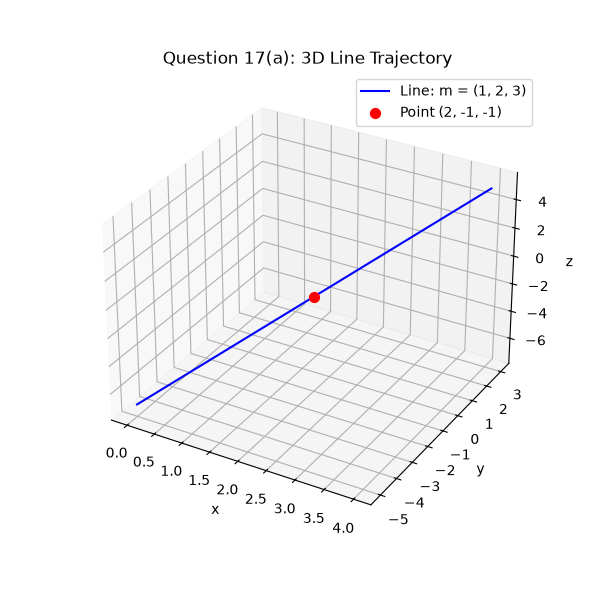
\includegraphics[width=0.6\textwidth]{figs/q17_fig}
			\caption{3D line direction and point representation.}
			\label{fig:q17_fig}
			\vspace{0.5em}
			\noindent\fbox{\parbox{\dimexpr\linewidth-2\fboxsep-2\fboxrule}{\hspace{2em}\textbackslash codes\textbackslash q17.py}}
		\end{figure}
		\item Present value formula $P = R \sbrak{\frac{1 - (1+i)^{-n}}{i}}$.
		Substituting $R = 500, i = 0.15, (1.15)^{-12} \approx 0.1869$:
		\begin{align}
			P = 500 \sbrak{\frac{1 - 0.1869}{0.15}} = 500 \times 5.4206 = \text{Rs. } 2710.30
		\end{align}
	\end{enumerate}
	
	\item \hfill
	\begin{enumerate}[label=(\alph*)]
		\item If the plane $x + y + z = \sqrt{3}\lambda$ touches the sphere $x^2 + y^2 + z^2 - 2x - 2z - 6 = 0$, find the value of $\lambda$.
		\item An insurance company discovers $0.1\%$ of the population is involved in accidents. For 1000 policy holders, find the probability that not more than 5 are involved next year. [Use $e^{-1} = 0.368$]
	\end{enumerate}
	\solution
	\begin{enumerate}[label=(\alph*)]
		\item Rewriting the equation of the sphere by completing squares:
		\begin{align}
			(x-1)^2 + y^2 + (z-1)^2 - 1 - 1 - 6 = 0 \implies (x-1)^2 + y^2 + (z-1)^2 = 8
		\end{align}
		The center of the sphere is $\vec{c} = \myvec{1 \\ 0 \\ 1}$ and radius $r = \sqrt{8} = 2\sqrt{2}$.
		The given plane equation is $x + y + z - \sqrt{3}\lambda = 0$ with normal vector $\vec{n} = \myvec{1 \\ 1 \\ 1}$.
		Applying the tangency condition from \eqref{eq:sphere_plane_tangency_formula}:
		\begin{align}
			\frac{\abs{1(1) + 1(0) + 1(1) - \sqrt{3}\lambda}}{\sqrt{1^2 + 1^2 + 1^2}} = 2\sqrt{2} \implies \frac{\abs{2 - \sqrt{3}\lambda}}{\sqrt{3}} = 2\sqrt{2}
		\end{align}
		Simplifying:
		\begin{align}
			\abs{2 - \sqrt{3}\lambda} = 2\sqrt{6} \implies 2 - \sqrt{3}\lambda = \pm 2\sqrt{6} \implies \lambda = \frac{2 \mp 2\sqrt{6}}{\sqrt{3}} = \frac{2\sqrt{3} \mp 6\sqrt{2}}{3}
		\end{align}
		\begin{figure}[H]
			\centering
			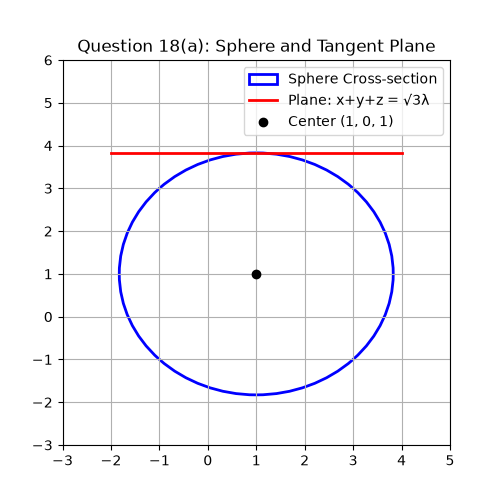
\includegraphics[width=0.6\textwidth]{figs/q18_fig}
			\caption{Sphere and tangent plane representation.}
			\label{fig:q18_fig}
			\vspace{0.5em}
			\noindent\fbox{\parbox{\dimexpr\linewidth-2\fboxsep-2\fboxrule}{\hspace{2em}\textbackslash codes\textbackslash q18.py}}
		\end{figure}
		\item Poisson PMF with $\lambda_{P} = np = 1000 \times 0.001 = 1$:
		\begin{align}
			p_X(X \le 5) = \sum_{k=0}^{5} \frac{0.368}{k!} = 0.368 \times 2.7167 \approx 0.9997
		\end{align}
	\end{enumerate}
	
	\item \hfill
	\begin{enumerate}[label=(\alph*)]
		\item Three forces $\vec{P}, \vec{Q}$ and $\vec{R}$ acting at a point are in equilibrium. The angle between $\vec{P}$ and $\vec{R}$ is double the angle between $\vec{P}$ and $\vec{Q}$. Prove that $R^2 = Q(Q-P)$.
		\item The horizontal roadway of a bridge $AB$, $12\text{ m}$ long, weight $56000\text{ N}$ and rests on two supports at its ends. What is the pressure on each support when a lorry of weight $33600\text{ N}$, starting from $A$, is at a point two-third of the way on the bridge?
		\item A housewife wishes to mix up two kinds of foods $X$ and $Y$ in such a way that mixture contains at least 10 units of vitamin A, 12 units of vitamin B and 8 units of vitamin C.
		\begin{center}
			\begin{tabular}{|c|c|c|c|}
				\hline
				Food & Vitamin A & Vitamin B & Vitamin C \\ \hline
				X & 1 & 2 & 3 \\
				Y & 2 & 2 & 1 \\ \hline
			\end{tabular}
		\end{center}
		If one kg of food $X$ costs Rs. 6 and one kg of food $Y$ costs Rs. 10, find the least cost of the mixture which will produce the desired diet.
		\item A manufacturer makes two types of cups, A and B. Three machines are required to manufacture the cups and the time in minutes required by each is as given below:
		\begin{center}
			\begin{tabular}{|c|c|c|c|}
				\hline
				Type of Cup & \multicolumn{3}{c|}{Machines} \\ \hline
				& I & II & III \\ \hline
				A & 12 & 18 & 6 \\
				B & 6 & 0 & 9 \\ \hline
			\end{tabular}
		\end{center}
		Each machine is available for a maximum period of 6 hours per day. If the profit on each cup A is 75 paise, and on B it is 50 paise, show that 15 cups of type A and 30 cups of type B should be manufactured per day to get the maximum profit.
	\end{enumerate}
	\solution
	\begin{enumerate}[label=(\alph*)]
		\item Expressing static equilibrium $\vec{P} + \vec{Q} + \vec{R} = \vec{0}$ in component scalar form:
		\begin{align}
			P + Q\cos\theta + R\cos 2\theta &= 0 \\
			Q\sin\theta - R\sin 2\theta &= 0 \implies \cos\theta = \frac{Q}{2R}
		\end{align}
		Substituting $\cos\theta = \frac{Q}{2R}$ into the $x$-component equation:
		\begin{align}
			P + Q\brak{\frac{Q}{2R}} + R\brak{2\frac{Q^2}{4R^2} - 1} = 0 \implies R^2 = Q(Q-P)
		\end{align}
		\begin{figure}[H]
			\centering
			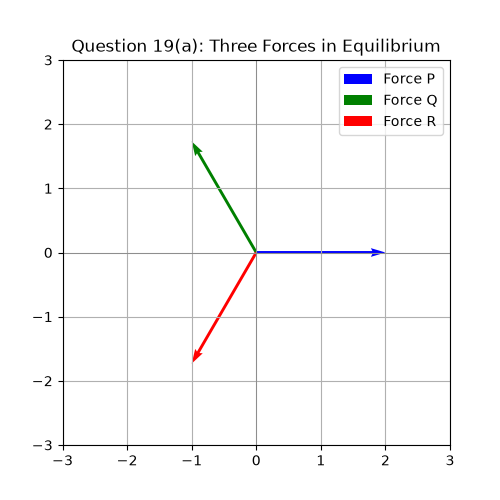
\includegraphics[width=0.6\textwidth]{figs/q19_fig}
			\caption{Three forces in static equilibrium.}
			\label{fig:q19_fig}
			\vspace{0.5em}
			\noindent\fbox{\parbox{\dimexpr\linewidth-2\fboxsep-2\fboxrule}{\hspace{2em}\textbackslash codes\textbackslash q19.py}}
		\end{figure}
		\item Vertical force balance $R_A + R_B = 56000 + 33600 = 89600\text{ N}$. Taking moments about $A$:
		\begin{align}
			12 R_B = (56000 \times 6) + \brak{33600 \times 8} \implies R_B = 50400\text{ N}, \quad R_A = 39200\text{ N}
		\end{align}
		\item Minimize $Z = 6x + 10y$ subject to:
		\begin{align}
			x + 2y \ge 10, \quad 2x + 2y \ge 12 \implies x + y \ge 6, \quad 3x + y \ge 8, \quad x, y \ge 0
		\end{align}
		Evaluating corner points of the feasible region yields minimum cost $Z = \text{Rs. } 52$ at $x = 2\text{ kg}, y = 4\text{ kg}$.
		\item Maximize profit $Z = 0.75x + 0.50y$ subject to machine hour constraints (converting 6 hours to 360 minutes):
		\begin{align}
			12x + 6y \le 360 \implies 2x + y \le 60 \\
			18x \le 360 \implies x \le 20 \\
			6x + 9y \le 360 \implies 2x + 3y \le 120
		\end{align}
		Corner point analysis of the feasible polygon yields maximum daily profit $Z = \text{Rs. } 26.25$ at $x = 15$ cups of type A and $y = 30$ cups of type B.
	\end{enumerate}
	
\end{enumerate}